\chapter{Petri网基本理论}
本章为本文的理论研究的基础,主要介绍了Petri网概念与特性,包过:Petri网定义、Petri网模型结构、Petri网可达图和Petri网特性;
介绍了Petri网在不同领域的应用;
介绍了一系列Petri网的调度方法;
最后介绍了一系列时间网。
为后续章节提供理论支持。
\section{Petri网概念与特性}
    Petri网是一种描述离散事件系统的数学模型,它既可以用数学定义形式化地表示,也可以用图形形象化地表示。
    使用Petri网建立的模型具有简单、易懂、可操作性强等特点,能够很直观地表述出各类实际系统模型中并发、依赖、冲突、死锁等情况。
    Petri网既可用于结构分析又可用于行为分析,因此在各个领域均有广泛应用\cite{24143}\cite{7426418}\cite{wu:hal-00735482}。

    \subsection{Petri网定义}
    一个Petri网中通常是由两种节点组成的图,这两种节点分别为:库所(Place),变迁(Transition),
    每个元素含义与功能各不相同:库所中存放托肯(Token),托肯表示系统的资源;
    变迁一般代表能够改变系统状态的某种事件,变迁执行一种称为发射的操作,变迁发射后会改变库所中的资源的状态,从而改变系统的状态;
    变迁和库所间通过有向弧(Arc)连接,如果有向弧从库所指向变迁,意味着变迁发射后会从库所中取走一定数目的托肯,如果有向弧从变迁指向库所,意味着变迁发射后会放入一定数目的托肯进库所;
    Petri网也可以图形表示,
    在图形上分别用矩形($\Box $)表示变迁、圆圈($\bigcirc $)表示库所,某些变迁和托肯间会通过箭头连接,箭头($\leftarrow$)表示有向弧。

    \textbf{定义2.1}\cite{murata1989petri}\textbf{:}
    Petri网可以用一个四元组进行数学表示,四元组的元素分别为:库所集合、变迁集合、有向弧集合、有向弧上到权值的映射关系,即$N=(P,T,F,W)$,
    $P=\{p_{0},p_{1},p_{2},...,p_{i}\}$,$i \in \mathbb{N}^{+}$,是一个限非空的库所集合;
    $T=\{t_{0},t_{1},t_{2},...,t_{j}\}$,$j \in \mathbb{N}^{+}$,也是一个限非空的变迁集合;
    这两个集合不存在相交部分,因为Petri网中的一个元素不能即是库所又是变迁,即$P \neq \emptyset , T \neq \emptyset, P \cap T=\emptyset$。
    库所和变迁间通过有向弧连接,即
    $F \subseteq(P \times T) \cup(T \times P)$。
    弧上带有权值,即i
    $W:(P \times T) \cup(T \times P) \rightarrow \mathbb{N}$,对于任意$w \in W$,$w=1$,如果存在某个权值$w$不为1,则称这个网为一般网。
i
    \textbf{例2.1}\hspace{0.5em}
    如图2.1就是某Petri网的图形表示,他的数学表示为:$N = (P, T, F, W)$,$P =  \{p_{1}, p_{2}, p_{3}, p_{4}, p_{5}, p_{6}\}$为此Petri网库所的集合,
    此Petri网有6个库所;
    $T = \{t_{1}, t_{2}, t_{j3}, t_{4}\}$ 为此Petri网变迁的集合,
    此Petri网有4个变迁;
    \begin{equation}
        \begin{aligned}
            F = \{(p_{1}, t_{2}), (t_{1}, p_{1}), (p_{2}, t_{3}), (t_{2}, p_{2}), (p_{3}, t_{4}), \\(t_{3}, p_{3}), (p_{4},t_{1} ), (t_{2},p_{4} ), (p_{5}, t_{3}), (t_{4}, p_{5}), (p_{6}, t_{1}), (t_{4}, p_{6})\}
        \end{aligned}
        \nonumber 
    \end{equation}为此Petri网有向弧集合,
    有向弧的权值为:$W(p_{1}, t_{2}) = W(t_{1}, p_{1}) = W(p_{2}, t_{3}) = W(t_{2}, p_{2}) = W(p_{3}, t_{4}) = W(t_{3}, p_{3}) = W(p_{4},t_{1}) = W(t_{2},p_{4} ) = W(p_{5}, t_{3} ) = W(t_{4}, p_{5} ) = 1$,
    $W(t_{4}, p_{6})=W(p_{6}, t_{1}) = 2$。
    因为这个网中的有向弧上的权值并不全为1,而是存在2个有向弧上权值为2,所以是一个一般网。
    
    \begin{figure}[H]
        \centering
        % Requires \usepackage{graphicx}
        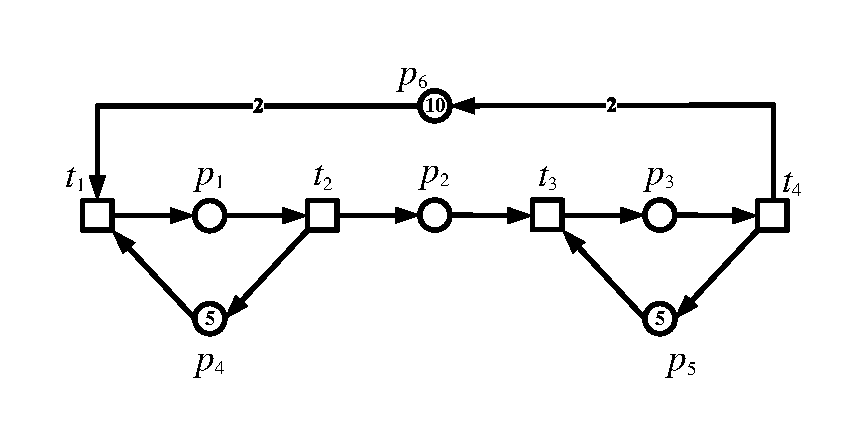
\includegraphics[scale=0.8,angle=0]{figures/figure2-1.pdf}\\
        \caption{一个一般Petri网模型}
    \end{figure}

    \textbf{定义2.2}\cite{Liu2013}\textbf{:}
    对于某Petri网$N = (P, T, F, W)$,在此网中的任意一个节点$m \in P \cup T$,分别在其前后打点,表示此节点的前置节点集合和后置节点集合,
    记$^{\bullet}m$为节点$m$的前置集合,$^{\bullet} m = \{n \in P \cup T|(n, m) \in F\}$;
    记$m^{\bullet}$为节点$m$的后置集合,$m^{\bullet} = \{n \in P \cup T|(m, n) \in F\}$,
    如果节点$m \in P$,那么$^{\bullet}m \subseteq T$,$m^{\bullet} \subseteq T$,
    如果节点$m \in T$,那么$^{\bullet}m \subseteq P$,$m^{\bullet} \subseteq P$,
    相应地,将全部节点的集合记作$M \subseteq (P \cup T)$,则节点集合满足$^{\bullet}M = \cup _{m \in M} {^\bullet}m$,$M^{\bullet} = \cup_{m \in M} m^{\bullet}$。
    若满足$\forall i\in \mathbb{N}^+ = \{1, 2,...,n-1\}$,$y_{i+1} \in y_i^{\bullet}$。 此节点序列$m_{1}, m_{2},..., m_{i},...,m_{j}$ 即为Petri网$N$的路径,其中$m_{i} \in P \cup T$。
    如果在这条路径中除了$m_{1}$和$m_{j}$以外,所有的节点都不相同,并且$m_{1} = m_{j}$,即此节点序列的首尾相同,遍历此序列最终会回到原点,因此此序列构成一条回路,此Petri网被称为一条简单回路。
    
    在定义2.2中,
    如果$m$表示库所,此库所的前置集$^{\bullet} m$中的变迁称为输入变迁,
    此库所的后置集$m^{\bullet}$中的变迁称为输出变迁集。
    如果$m$表示变迁,此变迁的前置集$^{\bullet} m$中的库所称为输入库所,
    此变迁的后置集$^{\bullet} m$中的库所称为输出库所。

    \textbf{例2.2}\hspace{0.5em}
    如图2.2所示,是一个简单的Petri网模型,此网P中所有库所($p_{1},p_{2},p_{3},p_{4},p_{5}$) \\ 的前置变迁集合与后置变迁集合为:
    $^\bullet p_1 = \{t_1\}$,${p_1}^\bullet = \{t_2\}$,
    $^\bullet p_2 = \{t_2\}$,${p_2}^\bullet = \{t_3\}$,
    $^\bullet p_3 = \{t_3\}$,${p_3}^\bullet = \{t_4\}$,
    $^\bullet p_4 = \{t_2, t_4\}$,${p_4}^\bullet = \{t_1, t_3\}$,
    $^\bullet p_5 = \{t_4\}$,${p_5}^\bullet = \{t_1\}$。
    网模型中所有变迁($t_{1},t_{2},t_{3},t_{4}$)的前置库所集合和后置库所集合为:
    $^\bullet t_1 = \{p_4, p_5\}$,${t_1}^\bullet = \{p_1\}$,
    $^\bullet t_2 = \{p_1\}$,${t_2}^\bullet = \{p_2, p_4\}$,
    $^\bullet t_3 = \{p_2, p_4\}$,${t_3}^\bullet = \{p_3\}$,
    $^\bullet t_4 = \{p_3\}$,${t_4}^\bullet = \{p_4, p_5\}$。
    对于一组节点序列:$p_1, t_2, p_2, t_3, p_3, t_4, p_4, t_1, p_1$就是此Petri网的一条路径,因为此路径的首尾相同,其他节点均不相同,因此这是一条简单回路。
    
    \begin{figure}[H]
        \centering
        % Requires \usepackage{graphicx}
        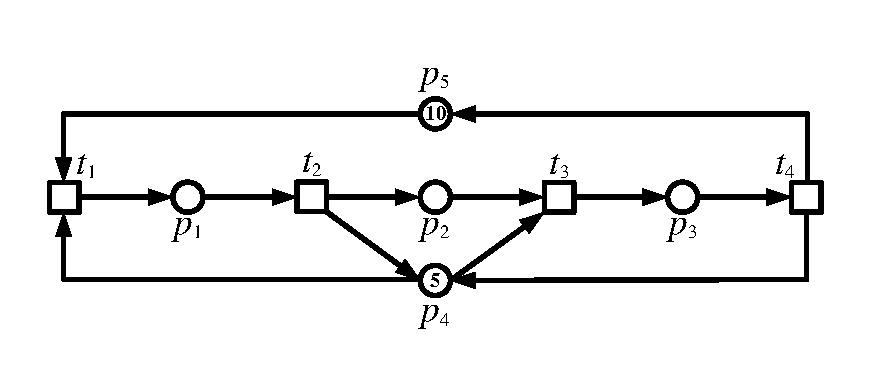
\includegraphics[scale=0.8,angle=0]{figures/figure2-2.pdf}\\
        \caption{一个Petri网模型}
    \end{figure}

    \textbf{定义2.3}\cite{murata1989petri}\textbf{:}
    一个Petri网$N = (P, T, F, W)$,如果满足条件$\forall x, y \in (P \cup T)$,$W(x, y)> 0$,$W(y, x) = 0$,则将此Petri网称为一个纯网(pure net)。
    
    要判断一个Petri网是否是纯网,可以使用关联矩阵,以及前置矩阵和后置矩阵。$[N]$是$|P| \times |T|$的一个整数矩阵。$[N]$可以进一步进行拆分为$[N]^+$和$[N]^-$ ,对其进行矩阵运算得到$[N]$,运算公式为$[N]=[N]^+ - [N]^- $。其中$\forall t \in T$,$\forall p \in P$,$[N]^+(p,t) = W(t, p)$,$[N]^-(p,t) = W(p, t)$。
    
    \textbf{例2.3}\hspace{0.5em}
    图2.2所示的Petri网模型,所有的有向弧只有一个方向,因此此Petri网没有自环,是一个纯网。

    对于图2.2中所示的Petri网中,将其库所变迁的关系分解为如下三个矩阵,其中$[N]^+$为输入关联矩阵,$[N]^-$为输出关联矩阵,$[N]$为关联矩阵。
    \begin{equation}\label{equaN}
    [N^+]=\begin{pmatrix}
    0&1&0&0\\
    0&0&1&0\\
    0&0&0&1\\
    1&0&1&0\\
    1&0&0&0
    \end{pmatrix}\ \ \ \ \ \ \
    [N^-]=\begin{pmatrix}
    1&0&0&0\\
    0&1&0&0\\
    0&0&1&0\\
    0&1&0&1\\
    0&0&0&1
    \end{pmatrix}\ \ \ \ \ \ \
    [N]=\begin{pmatrix}
    -1&1&0&0\\
    0& -1&1&0\\
    0 &0&-1&1\\
    1&-1 &1&-1\\
    1&0&0&-1
    \end{pmatrix}
    \end{equation}

    在上述所示的关联矩阵中,$[N^+]_{(p_1,t_2)}=1$,意味这如果此Petri网发射$t_2$变迁,会往库所$p_1$中放入1个托肯,
    $[N^-]_{(p_1,t_2)}=0$,意味着发射$t_2$变迁,不会往$p_1$取走托肯,
    前两个关联矩阵复合后得到的$[N](p_1,t_2)=1$意味着如果此Petri网发射$t_2$变迁,库所$p_1$中的托肯数量会加1。

    \textbf{定义2.4}\cite{Liu2010}\textbf{:}
    Petri网$N = (P,T,F,W)$中任意标识$M$都是一个维数与库所数相同的自然数向量。$(P,T,F,W,M_{0})$也可以直接记为$(N,M_{0})$,$N$表示Petri网的结构,$M_{0}$称为网系统的初始标识,表示Petri网的初始状态。

    \textbf{例2.4}\hspace{0.5em} 图2.2所示的Petri网,此Petri网的初始标识向量为:$M_{0}=(0,0,0,5,10)^{T}$,
    也可以使用与库所有关的多项式表示,
    即当表示向量对应库所的数值作为系数,乘上对应库所,再求和组成的多项式
    对于初始标识$M_{0}$,此标识向量为:
    $M_{0}=5p_{4}+10p_{5}$。

    \textbf{定义2.5}\cite{Liu2013}\textbf{:}
    对于某Petri网,如果在当前标识$M$下,如果某个变迁$t$满足$\forall p\in{^\bullet t}, M(p) \geq W(p,t)$,
    则称变迁$t$在标识$M$下是使能的,并将其记作$M[t\rangle$。一般来说,Petri网库所是有容量限制的,如果变迁$t$ 在标识$M$下是使能的,并且变迁$t$发射后,不会超过库所容量的限制,即满足$\forall p \in t^{\bullet}, M(p)+W(t,p) \leq MAX(p)$,
    则此变迁能被安全发射,其中$MAX(p)$表示库所$p$中能够存放的最多托肯的数量,也就是库所容量。变迁$t$ 发射后会改变Petri网模型中各库所中托肯的状态,因此Petri网的状态也就被改变了,从而产生一个新的Petri网的标识,在可达图中新标识是原标识的后继节点,两标识通过变迁连接,新标识的计算公式为$M^{\prime}(p)=M(p)-W(p,t)+W(t,p)$,
    原标识与新标识的关系记为$M[t\rangle M^{\prime}$,表示可达状态$M$可以通过发射变迁$t$到达可达状态$M^{\prime}$。

    \textbf{例2.5}\hspace{0.5em}
    在图2.2所示的Petri网模型中,初始标识为$M_{0}=5p_{4}+10p_{5}$,表示库所$p_{4}$中有5个托肯,库所$p_{5}$中有10个托肯,在此标识下变迁$t_1$是可以安全发射的,
    记作$M_0 [t_1\rangle$,表示变迁$t_1$在状态$M_{0}$下发射后既不会使库所中的托肯数为负数,也不会超过库所容量。
    变迁$t_1$的前置库所集合为$^\bullet t_1 = \{p_4, p_5\}$,分别判定$p_4$,$p_5$两个库所是否能安全地取走托肯:$M_0(p_4)=5 > W(p_4, t_1)=1$,$M_0(p_5)=10 > W(p_5, t_1)=1$,这两个库所中都有足够多的托肯数发射变迁$t_1$,所以变迁$t_1$能够发射,
    在发射后,库所$p_1$的托肯数更新为$M_1(p_1)=M_0(p_1)-W(p_1, t_1)+W(t_1, p_1)=1$,
    库所$p_4$的托肯数更新为$M_1(p_4)=M_0(p_4)-W(p_4, t_1)+W(t_1, p_4)=4$, 
    库所$p_5$的托肯数更新为$M_1(p_5)=M_0(p_5)-W(p_5, t_1)+W(t_1, p_5)=9$。
    此Petri网的标识从$M_0=5p_4+10p_5$更新为$M_1=p_1+4p_4+9p_5$,
    $M_0$可以通过发射$t_1$到达$M_1$,记作$M_0[t_1\rangle M_1$。

    \textbf{定义2.6}\cite{Liu2013}\textbf{:}
    如果对于Petri网$N$,初始标识$M$发射某变迁后能够到达新标识$M^{\prime}$,
    则称$M$到$M^{\prime}$是可达的,记为$M[\delta\rangle M_{n}$,
    如果$M[t_{1}\rangle M_{1}[t_{2}\rangle M_{2}\ldots M_{n-1}[t_{n}\rangle M_{n}$,
    意味着$t_1$,$t_2$可以被连续发射,
    则变迁序列$\delta=t_{1}t_{2}\dots t_{n-1}t_{n}$ 为网中的一个可发射的序列,
    $M_{1},M_{2},\dots,M_{n-1},M_{n}$为Petri网$N$的可达标识。
    因为这两个变迁均可发射,所以可以使用下述状态方程直接计算发射这两个变迁后的标识,
    $M_{n}=M+[N]\overrightarrow{\delta}$,其中将$\overrightarrow{\delta}$: $T\rightarrow \mathbb{N}$称作是计数型整数向量,在发射序列$\delta$中变迁$t$发射的次数和可以用$\overrightarrow{\delta}(t)$来表示。

    \textbf{例2.6}\hspace{0.5em}
    如图2.2所示,在此Petri网$N$中发射一条变迁序列$\delta=t_1t_2t_3t_4$,其中$\overrightarrow{\delta}= [1 \quad 1 \quad 1 \quad 1]^T$称为Petri网$N$的发射向量。
    通过发射变迁序列$\delta$产生了新的可达标识$M'$ ,此过程可以使用下述状态方程表示:
    
    \begin{equation}\label{equaM}
    M_n=M_0+[N]\overrightarrow{\delta}=\begin{pmatrix}
    0\\
    0\\
    0\\
    5\\
    10
    \end{pmatrix}+\begin{pmatrix}
    -1&1&0&0\\
    0& -1&1&0\\
    0 &0&-1&1\\
    1&-1 &1&-1\\
    1&0&0&-1
    \end{pmatrix}\begin{pmatrix}
    1\\
    1\\
    1\\
    1
    \end{pmatrix}=
    \begin{pmatrix}
    0\\
    0\\
    0\\
    5\\
    10
    \end{pmatrix}=M_0
    \end{equation}
    
    此变迁序列发射完后,又回到了初始标识$M_0$,这是因为这个发射序列正好是此Petri网的一条完整的回路,并且所有的弧上权值均为1。

    \textbf{定义2.7}\cite{murata1989petri}\textbf{:}
    对于一个Petri网$N$,从某标识$M$出发,能够通过变迁序列到达的所有标识的集合记为$M[\rangle$。
    如果是从初始标识$M_{0}$出发,其可达标识集为$M_{0}[\rangle$,也可以记为$R(N,M_{0})$。
    在标识$M_{0}$下,如果$\exists M^{\prime}\in R(N,M)$ 使得$M^{\prime}[t\rangle$,
    当且仅当对$\forall M \in R(N,M_{0})$成立;
    对于变迁集中的所有变迁,即$\forall t \in T$,
    则变迁$t$是活的,如果存在某变迁在初始标识$M_0$下是活的,
    则网$(N,M_{0})$是活的(live);
    对于初始标识下所有的可达标识$\forall M \in R(N,M_{0})$,
    如果$\nexists t \in T$ ,$M^{\prime}[t\rangle$ ,
    则此Petri网$(N,M_{0})$是无死锁的(deadlock-free)。

    \textbf{例2.7}\hspace{0.5em}
    判定2.3所示的三个Petri网的活性。

    \begin{figure}[H]
        \centering
        % Requires \usepackage{graphicx}
        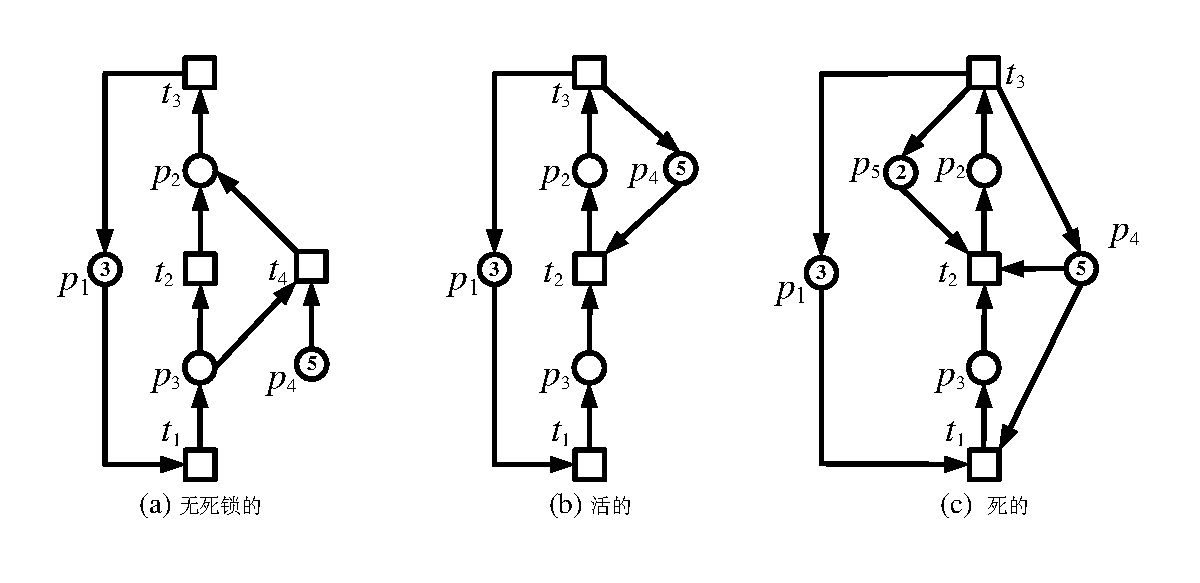
\includegraphics[scale=0.7,angle=0]{figures/figure2-3.pdf}\\
        \caption{一个Petri网活性示例}
    \end{figure}

    图2.3(a)中的Petri网没有死锁标识,变迁变迁$t_{4}$不是活的,因此称此Petri网是无死锁的;
    图2.3(b)中的Petri网所有变迁都是活的,因此称此Petri网活的;
    图2.3(c)中的Petri网存在死锁标识,因此称此Petri网是死的。
    \subsection{Petri网模型结构}
    使用Petri网建模,可以很直观地描述出模型结构\cite{petri},本小节将对Petri网中的四种结构模型:顺序、并发、冲突、混淆进行详细介绍。
    \subsubsection{顺序关系}
    在某标识下,如果某变迁发射,可以时原本不能使能的变迁使能,也就是说变迁可以顺序发射下去,则称这两个变迁在这个标识下是顺序关系,如图2.4(a)所示。

    \textbf{定义2.8}\cite{petri}\textbf{:}
    对于标识$M$,$\exists $变迁$t_{1}$、$t_{2}$,$M[t_1\rangle M'$,$\lnot M[t_2\rangle$,$M'[t_2\rangle$,
    变迁$t_{1}$、$t_{2}$在标识$M$下为顺序关系。
    \subsubsection{并发关系}
    在某标识下,如果两个变迁都可以使能,并且其中任何一个变迁发射都不会使另一个变迁不使能,就称这两个变迁为并发关系。并发关系下的两个变迁,是可以独立发射的,如图2.4(b)所示。

    \textbf{定义2.9}\cite{petri}\textbf{:}
    对于标识$M$,$\exists $变迁$t_{1}$、$t_{2}$,$M[t_1\rangle$,$M[t_2\rangle$,并且$M[t_1\rangle M_1\Rightarrow M_1[t_2\rangle$,$M[t_2\rangle M_2\Rightarrow M_2[t_1\rangle$,
    变迁$t_{1}$、$t_{2}$在标识$M$下为并发关系。
    \subsubsection{冲突关系}
    与并发关系正好相反,如果在某标识下,两个使能变迁发射任何一个,都会使另一个无法使能,则称这两个变迁在这个标识下是冲突关系,如图2.4(c)所示。

    \textbf{定义2.10}\cite{petri}\textbf{:}
    对于标识$M$,$\exists $变迁$t_{1}$、$t_{2}$,$M[t_1\rangle$,$M[t_2\rangle$,并且$M[t_1\rangle M_1\Rightarrow M_1[t_2\rangle$,$M[t_2\rangle M_2\Rightarrow M_2[t_1\rangle$,
    变迁$t_{1}$、$t_{2}$在标识$M$下为并发关系。
    \subsubsection{混淆关系}
    如果一个Petri网中同时存在并发和冲突两种关系的变迁,并且并发关系的变迁发射后会时冲突关系消失。在这种情况下是无法判断出冲突关系是否出现过的,因此称变迁间的这个关系为混淆关系,如图2.4(d)所示。

    \begin{figure}[H]
        \centering
        % Requires \usepackage{graphicx}
        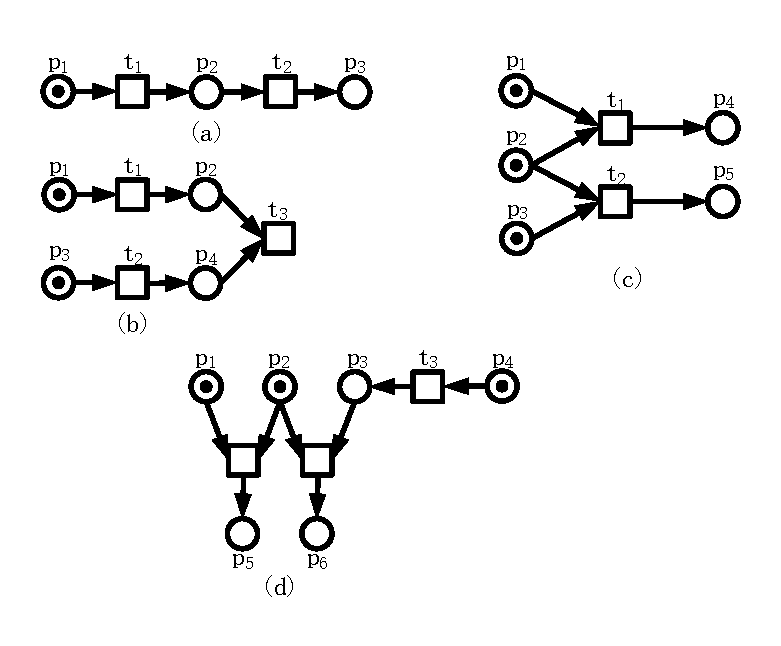
\includegraphics[scale=0.7,angle=0]{figures/figure2-4.pdf}\\
        \caption{Petri网模型结构}
    \end{figure}

    \subsection{Petri网可达图}
    本文所研究的调度算法需要在Petri网可达图中搜索一条路径,所以本节将要介绍Petri网可达图(reachability graph)。
    可达图是分析Petri网的重要工具,而且不论是何种Petri网都有可达图。在可达图中可以清晰直观地看出不同标识是如何通过变迁转换的。
    给出Petri网以及此Petri网的初始标识,便可确定这个Petri网的可达图。
    利用Petri网可达图可以分析此Petri网所描述的离散事件系统的可达性、有界性、活性、安全性等一些列重要性质,是Petri网理论中十分有用的分析工具。

    \textbf{定义2.11}\cite{li2009deadlock}\textbf{:}
    记一个Petri网$(N, M_{0})$的可达图为$RG(N, M_{0})= (U, S)$,可达图中包含该网模型的所有可达标识以及可达标识之间的变迁关系,可达图是一个有向图。
    其中,可达图中用圆圈表示节点,
    用$U= R(N, M_{0})$代表网的全部可达标识;可达图中节点之间的有向连接弧用集合$S= \{(M, t, M^{\prime})\mid M^{\prime} \in R(N, M_{0})$,$M[t\rangle M^{\prime}\}$来表示,
    弧上标注了对应的变迁,用来说明从一个可达标识到达另一个可达标识所需要发射的变迁,也就是可达标识之间的映射关系。

    可达图算法与传统的图遍历算法并无本质上的区别。
    通过算法2.1\cite{zby2019}可以得到一个Petri网的可达图:

    \begin{algorithm}[H]
        \caption{可达图算法}
        \label{alg2-1}
        \begin{algorithmic}
            \Procedure {RG}{}
            \Require 一个标记的Petri网 $(N, M_{0})$。 \notag
            \Ensure 网模型的可达图。
            \State 可达图$RG(N,M_{0})$的开始点为初始标识$M_{0}$
            \State 一开始Petri网的全部可达标识没有被标记
            \State \textbf{while}\{有可达标识未被标记\}\textbf{do}
                
                \State \hspace{0.8cm} 对未被标记的可达标识$M$
                
                \State \hspace{0.8cm} 考虑可达标识$M$下每一个使能的变迁$t$,通过$M^{\prime}=M+[N](\cdot,t)$计算新的可达标识$M^{\prime}$
                
                \State  \hspace{0.8cm} \textbf{if}\{可达图$RG$中还没有添加新的可达标识$M^{\prime}$\} \textbf{then}
                
                \State \hspace{1.4cm}  将新的可达标识$M^{\prime}$添加到可达图中
                
                \State \hspace{1.4cm}  在$M$到$M^{\prime}$之间添加有向弧并标记为$t$
                
                \State \hspace{0.8cm} \textbf{end if}
                
                \State  \hspace{0.8cm} 标记可达标识$M$
                
            \State  \textbf{end while}
            \EndProcedure
        \end{algorithmic}
    \end{algorithm}

    对图2.2中的Petri网使用此算法求取可达图,为了减少可达标识数,将初始标识改为$(0,0,0,1,2)$,将得到如下可达标识:

    \begin{table}[H]
        \centering
        \begin{tabular}{|l|l|}
        \hline
            可达标识 & 使能变迁 \\ \hline
            $M_0:(0,0,0,1,2)$ & $t_1$ \\ \hline
            $M_1:(1,0,0,0,1)$ & $t_2$ \\ \hline
            $M_2:(0,0,1,0,1)$ & $t_4$ \\ \hline
            $M_3:(0,2,0,1,0)$ & $t_3$ \\ \hline
            $M_4:(0,1,1,0,0)$ & $t_4$ \\ \hline
            $M_5:(0,1,0,1,1)$ & $t_1$ $t_3$ \\ \hline
            $M_6:(1,1,0,0,0)$ & $t_2$ \\ \hline
        \end{tabular}
        \caption{图2.2中的Petri网可达图}
    \end{table}

    \subsection{Petri网特性}
    Petri网的特性包过可达性、有界性、活性、可逆性、可覆盖性和持续性\cite{jcj2003},可使用上一节提到的可达图分析Petri网的这些特性。
    本节将简略介绍上述特性的含义。
    \subsubsection{可达性}
    可达性将是本文调度算法部分最为关注的特性。如果存在某条变迁序列$\delta $,使得初始标识$M_0$按此变迁序列发射,能够到达标识$M'$,就说$M'$是从$M_0$可达的,记作$M_0[\delta\rangle M'$。
    如果$\delta $中只有一个变迁,则说$M'$是从$M_0$立即可达的。
    实际上调度算法所要做的就是找到一条最优的变迁序列。
    一个Petri网$N$的所有可达标识组成一个可达标识集,记作$R(N,M_0)$或$R(M_0)$。
    表2.1就是图2.2中的Petri网的可达标识集,这里面所有标识都是可达的。
    \subsubsection{有界性}
    有界指的是Petri网的可达标识数是有限的,也可以描述成Petri网从初始标识$M_0$开始任何一个可达标识中任意一个库所的托肯数都有界。
    实际的物理模型中许多是有界的,一般情况下库所指的是存放资源的场所,是有容量的。
    实际建模时一般会直接给出库所容量的约束。
    表2.1中只有7个可达标识,因此图2.2中的Petri网是有界的。
    \subsubsection{活性}
    Petri网的活性和Petri网中是否有死锁有相关性。如果可达图的任何子图中都存在一个标识能使变迁$t$使能,则说明变迁$t$是活的,如果所有变迁都是活的,则称Petri网是活的。
    如果Petri网是活的,则它一定没有死锁标识。
    图2.2中的Petri网就是活的。
    \subsubsection{可逆性}
    可逆性也和Petri网中是否有死锁有相关性。如果可达图中任意一个可达标识都可以通过发射某条变迁序列回到初始标识,则称Petri是可逆的。
    因此如果Petri网是可逆的,则它一定没有死锁标识。
    图2.2中的Petri网就是可逆的。
    \subsubsection{可覆盖性}
    对于标识$M$,如果Petri网可达图中存在标识$M'$,$M'$中每个库所的托肯数都比$M$的大,则说明$M$是可覆盖的。
    \subsubsection{持续性}
    具有持续性的Petri网,一旦某变迁使能了,那它会一直使能,直到发射此变迁为止。
    图2.2中的Petri网的$t_2$、$t_3$、$t_4$变迁都是可持续的。
\section{Petri网的应用}
    在解决柔性制造系统生成调度问题时,Petri网能够充分反应实际模型的各种特性,因此Petri网在此方面应用十分广泛。Petri网在柔性制造系统中的各种应用如图2.5所示。
    \begin{figure}[H]
        \centering
        % Requires \usepackage{graphicx}
        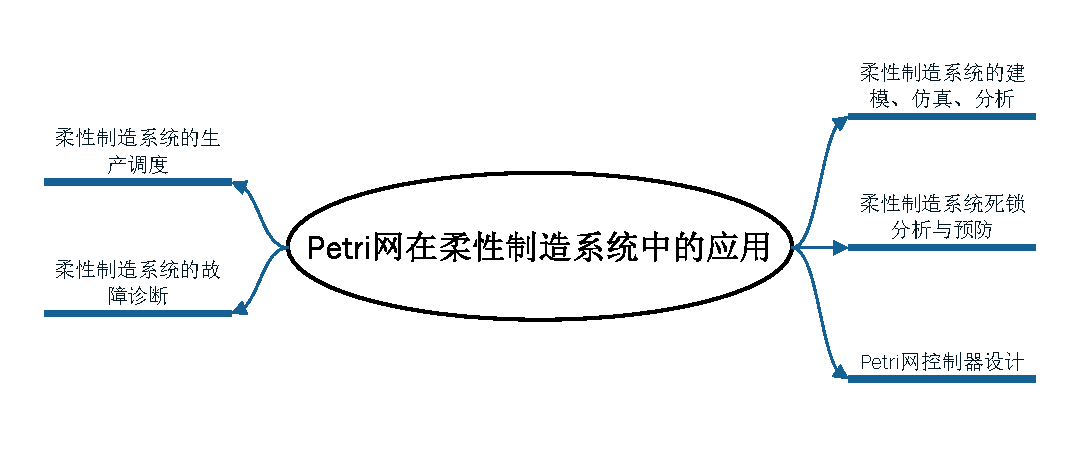
\includegraphics[scale=0.7,angle=0]{figures/figure2-5.pdf}\\
        \caption{Petri网在柔性制造系统中的各种应用}
    \end{figure}
\section{Petri网的调度方法}
    本文将着重研究基于蚁群算法的Petri网调度问题。这是一个群体智能的图搜索算法,在Petri网背景下,搜索的空间是可达图。
    因此本节将对各种图搜索算法进行介绍。
    本节介绍的算法分为两个大类:传统的图搜索算法、群体智能算法。
    \subsection{传统的图搜索算法}
        传统的图搜索算法具有很相似的结构。本类算法有两个集合,一个集合用于存放待扩展的节点,另一个集合用于存放已经扩展过的节点。
        每次从待扩展的节点集合中取出节点,基于此扩展新节点,如果新节点不在存放已经扩展过的节点集合中存在,则说明它有扩展的价值,将其放入待扩展的节点集合中。
        不断重复上述操作,直到找到终点,或者待扩展的节点集合为空。
        \begin{algorithm}[H]
            \caption{图搜索算法}
            \label{alg2-2}
            \begin{algorithmic}
                \Procedure {graphSearch}{}
                    \State 将起点存入待扩展的节点集合
                    \While{待扩展的节点集合不为空}
                        \State $curr \leftarrow$ 从待扩展的节点集合取出节点
                        \While{$curr$未完成扩展}
                            \State $next \leftarrow$ 扩展一个$curr$的后继节点
                            \If{$next$不在存放已经扩展过的节点集合中存在}
                                \State 将$next$放入待扩展的节点集合中
                            \EndIf
                        \EndWhile
                        \State 将$curr$放入已经扩展过的节点集合中
                    \EndWhile
                \EndProcedure
            \end{algorithmic}
        \end{algorithm}
        此后的一系列算法都是对从待扩展的节点集合取出节点这一步进行更精细的设计,从而改变图搜索的顺序。
        \subsubsection{深度优先搜索}
        深度优先搜索算法如果不发生回溯,每次扩展的节点都是相邻的,这意味着当前节点完成扩展后必须从它扩展出的新节点选择下一次要扩展的节点。
        因此因该选择先入后出的堆栈来实现待扩展的节点集合\cite{chen2019depth}\cite{liu2018improved}\cite{wu2017depth}\cite{zhang2016novel}\cite{chen2015improved}。
        \subsubsection{基于Petri网的启发式调度}
        此算法是深度优先搜索算法的一个子类,通过设计对当前节点更为精细的扩展顺序来实现。
        比如每次都以单步最优的策略进行扩展,则可将当前节点的后继节点按距离排序后放入待扩展的节点集合中。
        体现在Petri网中,即为每次都发生最短完工的变迁,此策略称为最早完工策略\cite{johnson1954optimal}\cite{wagner1959theory}\cite{winston1969production}\cite{mather1972production}\cite{graves1981production}。
        \subsubsection{广度优先搜索}
        广度优先搜索会一层层地扩展搜索树,因此需要按顺序依次扩展当前节点的后继节点。
        因此待扩展的节点集合应选取先进后出的队列进行实现\cite{cormen2009introduction}\cite{yang2019approximating}\cite{liu2015new}\cite{mehlhorn1999data}\cite{yu2015research}。
        \subsubsection{迪杰斯特拉算法}
        迪杰斯特拉算法与广度优先搜索算法类似,在大方向上也是一层层地扩展可达树。
        不同的是,迪杰斯特拉算法每次扩展的节点都是待扩展的节点集合中离原点距离最短的。
        因此迪杰斯特拉算法一定能求出全局的最短路径\cite{dijkstra1959note}\cite{cormen2009introduction}\cite{sedgewick1990algorithms}\cite{dijkstra1976discipline}\cite{brandes2005centrality}。
        \subsubsection{启发式搜索算法}
        此算法又称A星算法,是对迪杰斯特拉算法的进一步优化。
        此算法的待扩展的节点集合会对每一个进入集合的节点进行估计,
        估计的是经过此节点的最短路径的长度。
        此长度值$f$分为两部分:起点到当前点的最短路径长度$g$、当前节点到终点的最短路径长度$h$,
        $$
            f=g+h
        $$
        如果估计合理,$g$的值是确定的,因为每次扩展都会往最优解上走,$g$的值就是当前路径当前节点离原点的距离。
        因此$h$的值将是影响算法的关键。

        因为Petri网的启发式函数需要结合具体情况进行设计,而本文研究的蚁群算法是一种通用的图搜索算法,所以本文在算法章节并不对A星算法进行测试。
        而深度优先搜索和广度优先搜索策略太过简单,效果是不如其他更为精细的搜索机制的,因此本文将主要使用Petri网的启发式调度、迪杰斯特拉算法为传统搜索算法的代表进行测试\cite{hart1968formal}\cite{russell2010artificial}\cite{nash2011incremental}\cite{sturtevant2012benchmarks}\cite{botea2004near}。
    \subsection{群体智能算法}
        群体智能算法之间流程差异巨大,但本质思想是类似的。
        群体智能算法会并发地开启多条搜索路径,并提供某种正反馈机制把解往优的解上引导。
        \subsubsection{遗传算法}
            遗传算法大体流程为:

            1、将问题的解编码为染色体;

            2、对一系列染色体评价其适应度;

            3、按适应度大小淘汰一批染色体;

            4、从幸存的染色体中使用交叉操作生成新的染色体;

            5、重复进行上述操作一定轮次后对适应度最高的染色体进行解码,得到并输出解\cite{eiben2015evolutionary}\cite{whitley1994genetic}\cite{mitchell1996introduction}\cite{holland1975adaptation}\cite{goldberg1989genetic}。

            \begin{algorithm}[H]
                \caption{遗传算法}
                \label{alg2-3}
                \begin{algorithmic}
                    \Procedure {GA}{}
                        \State 随机生成一批染色体
                        \While{未到达迭代轮数或解未收敛}
                            \State 对一系列染色体评价其适应度
                            \State 按适应度大小淘汰一批染色体
                            \State 从幸存的染色体中使用交叉操作生成新的染色体
                        \EndWhile
                        \State 对适应度最高的染色体进行解码,得到并输出解
                    \EndProcedure
                \end{algorithmic}
            \end{algorithm}
            本文研究的蚁群算法无需考虑Petri网的具体结构,因此基因算法也应具备通用性。
            所以本基因算法训练的染色体为变迁的优先级,再使用传统图搜索算法按此优先级进行搜索求解。
            具体流程会在算法章节详细描述。
        \subsubsection{蚁群算法}
            蚁群算法与基因算法不同,它无需设计染色体编码方式,可直接应用于图搜索。
            蚁群算法的大体流程为:

            1、各蚂蚁根据图中信息素浓度并发搜索;

            2、所有蚂蚁搜索完成后按规则在图上更新信息素;

            3、重复进行上述操作一定轮次后输出探索到的最优解\cite{blum2003metaheuristics}\cite{li2015survey}\cite{colorni1992distributed}\cite{kennedy1995particle}\cite{dorigo2004ant}。

            \begin{algorithm}[H]
                \caption{蚁群算法}
                \label{alg2-4}
                \begin{algorithmic}
                    \Procedure {AntClonyOptimization}{}
                        \While{未到达迭代轮数或解未收敛}
                            \State 各蚂蚁根据图中信息素浓度并发搜索
                            \State 所有蚂蚁搜索完成后按规则在图上更新信息素
                        \EndWhile
                        \State 输出探索到的最优解
                    \EndProcedure
                \end{algorithmic}
            \end{algorithm}

            蚂蚁会在更优的路径上添加更多的信息素,并且有更大的概率走上信息素浓度高的路径。
            在此正反馈机制下,更优路径的信息素浓度会随算法运行逐步升高。

            传统蚁群算法在求解Petri网调度问题时,其性能会受网结构影响,本文对此提出了一系列优化思路。
\section{一系列时间网}
实际制造系统中,时间也是重要的因素。
如机械臂的运动、加工腔加工均需要消耗不同的时间,
产率是衡量调度策略优劣的重要指标,
要求取产率,则需要知道系统完成特定任务时的时间,
为了实现上述功能,将时间因素加入Petri网中。

Petri网由库所、变迁以及连接库所变迁的有向弧构成,库所中存有托肯。
常规的为Petri网添加时间因素的方式便是在以上四种组成部分上添加时间限制,
时间限制会影响到Petri网的使能逻辑。
时间限制添加在Petri网不同的组成部分上便形成了四种不同的时间网,
分别为:时间变迁网、时间库所网、时间弧网、时间托肯网。
    \subsection{时间变迁网}
    将时间限制以区间的形式添加到普通Petri网的变迁上,便形成了时间变迁网(Time Transition Petri Net,TTPN)。
    每个时间区间由两个值组成,分别为区间的左右端点。
    区间的左端点,称为静态最早发射时间(Static Earliest Firing Time,Static EFT),
    区间的右端点为静态最晚发射时间(Static Latest Firing Time,Static LFT)。
    当Petri网的某个变迁使能之后,它最少需要消耗静态最早发射时间,最多需要消耗静态最迟发射时间才能完成发射。

    \textbf{定义2.12}\cite{2013Time}\textbf{:}
    $I=[a,b]$是一个时间区间(time interval),其中:

    1. $a\in\mathbb{R}^{+},b\in\mathbb{R}\cup\infty$

    2. $a \le b$

    记$TI$为时间区间的集合,设$I_{1},I_{2} \in TI,I_{1}=[m,n],I_{2}=[p,q],c \in \mathbb{R}^{+}$,

    则时间区间与时间区间的运算方式为:$I_{1}+I_{2}=[m+p,n+q]$,

    时间区间与常数的运算方式为$I_{1}+c=[m+c,n+c],I_{1}-c=[max(m-c,0),max(n-c,0)]$,

    时间区间的最值运算为:$max(I_{1},I_{2})=[max(m,p),max(n,q)]$,
    
    $min(I_{1},I_{2})=[min(m,p),min(n,q)]$。

    表明时间区间经过一元和二元运算后,其结果仍为时间区间。

    \textbf{定义2.13}\cite{2013Time}\textbf{:}
    一个TTPN是一个六元组$Z=(P,T,F,W,M_{0},I)$,其中:

    1. 五元组$(P,T,F,W,M_{0})$是一个基本Petri网;

    2. $I:T \rightarrow (\mathbb{Q}_{0}^{+} \cup 0)\times (\mathbb{Q}_{0}^{+} \cup {\infty})$,并且$T$中的每个变迁$I(t)=(I_{1}(t),I_{2}(t))$,$0 \leq I_{1}(t) \leq I_{2}(t)$。

    \textbf{例2.8}\hspace{0.5em}
    如图2.6所示,此Petri网即为TTPN。在基本的Petri网中每个变迁上添加时间区间,可以得到如图的TTPN。
    变迁$t_{3}$处的时间区间为$[3,5]$则意味着$t_{3}$使能后,至少需要3个时间单位,才可能发射,但必须在5个时间单位之内进行发射。
    其他使能变迁上的时钟也在计时,因此逻辑与变迁$t_{3}$类似,如果变迁$t_1$也是使能变迁,则$t_1$必须在1个时间单位之前进行发射,但是此时还未到使能变迁$t_{3}$的最早发射时间,
    因此$t_1$必然先于$t_{3}$发射,
    综合来看$t_{3}$是不可能发射的。
    变迁的前置库所中的托肯被取走过,此变迁上的时钟才会被重置,
    否则会一直保持计时,
    因此当$t_{1}$发射后,$t_{3}$的时钟也会计时,如果$t_{1}$发射后下一个标识中$t_{3}$依然能使能,其等待的时间应减去一部分,而不需要再重新等3个时间单位才能发射。

    \begin{figure}[H]
        \centering
        % Requires \usepackage{graphicx}
        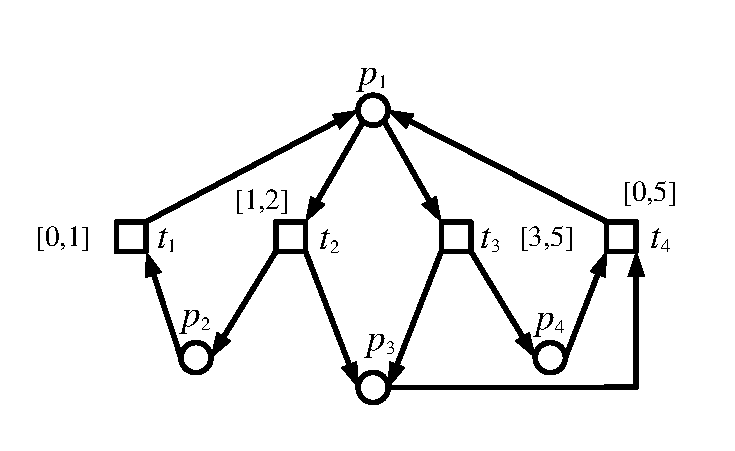
\includegraphics[scale=0.65,angle=0]{figures/figure3-1.pdf}\\
        \caption{一个TTPN模型}
    \end{figure}

    Petri网带有时间之后,原来的标识向量是无法表示此Petri网状态的所有信息。
    所以TTPN的标识除了包含库所中的托肯数,还包含了当前Petri网上每个变迁上的时钟信息。
    因此TTPN的标识需要包含两个元素,第一个元素描述库所状态,称作place-marking(简记作p-marking),
    第二个元素描述变迁状态,称为transition-marking(简记作t-marking)。
    p-marking即为普通Petri网的标识。
    t-marking表示了每个变迁上时钟的当前时间,如果此变迁不使能,则用符号$\nu$表示。

    \textbf{定义2.14}\cite{2013Time}\textbf{:}
    记$P$为时间网$Z$所有库所的集合,网$Z$的一个p-marking是一个从$P$到$\mathbb{N}$的映射:$P \rightarrow \mathbb{N}$。
    显然,时间网$Z$中的p-marking也是原网中的标识。

    \textbf{定义2.15}\cite{2013Time}\textbf{:}
    记$T$为时间网$Z$所有变迁的集合,时间网$Z$中的任意一个映射:$T \rightarrow \mathbb{R}_{0}^{+} \cup \{\nu\}$就是一个t-marking。

    \textbf{定义2.16}\cite{2013Time}\textbf{:}
    记$Z=(P,T,F,W,M_{0},I)$为一个时间Petri网,$m$为$Z$的一个p-marking,$h$为$Z$的一个t-marking,$Z$的一个状态为一个二元组$z=(m,h)$且:

    1. $\forall t ((t \in T \wedge t^{-} \nleq m) \rightarrow h(t) = \nu)$;

    2. $\forall t ((t \in T \wedge t^{-} \leq m) \rightarrow (h(t) \in \mathbb{R}_{0}^{+} \wedge h(t) \leq LFT(t)))$;

    状态$z_{0}=(m_{0},h_{0})$为时间网$Z$的初始状态,其中:

    $h_{0}(t)= \bigg \{\begin{array}{ll}
    0 & if \quad t^{-} \leq m_{0} \\
    \nu & if \quad t^{-} \nleq m_{0}
    \end{array}.$

    以上是时间网的静态特性。
    正如普通Petri网的动态特性是由发射规则所决定的,时间网的状态也与发射规则有关,时间网的当前状态会因为当前的p-marking或者t-marking的变化而改变。
    普通Petri网的p-marking会随着变迁的发射而改变,在时间网中,变迁的发射通常不仅改变当前的p-marking,也会改变t-marking。除了变迁的发射,t-marking也会随着时间的流逝而改变。

    \textbf{定义2.17}\cite{2013Time}\textbf{:}
    在时间网$Z=(P,T,F,W,M_{0},I)$中,变迁$t$在状态$z=(m,h)$下准备好发射的条件是:

    1. $t$在原网的标识$m$下是使能的,且$t^{-} \leq m$;

    2. $h(t) \geq EFT(t)$。

    \textbf{定义2.18}\cite{2013Time}\textbf{:}
    记$\hat{t}$和$z=(m,h)$分别为时间网$Z=(P,T,F,W,M_{0},I)$的一个变迁和一个状态,变迁$\hat{t}$能够在状态$z$下发射的条件是$\hat{t}$已经满足准备好发射的条件,
    记作$z \stackrel{\hat{t}}{\longrightarrow} $。$\hat{t}$发射之后,网$Z$的状态从$z$改变到$z^{'}=(m^{'},h^{'})$,记作$z \stackrel{\hat{t}}{\longrightarrow} z^{'}$,其中:

    1. $m^{'}=m+ \Delta \hat{t}$;

    2. $\forall t (t \in T \longrightarrow h^{'}(t)= \bigg \{\begin{array}{ll}
    \nu & if \quad t^{-} \nleq m^{'} \\
    h(t) & if \quad t^{-} \leq m \wedge t^{-} \leq m^{'} \wedge ^{\bullet}t \cap ^{\bullet}\hat{t} = \emptyset \wedge t \neq \hat{t} \quad )\\
    0 & otherwise
    \end{array}.$

    根据上述的定义,TTPN的每个变迁上都有一个时钟。
    此变迁使能以后,它上面的时钟开始计时,达到此变迁的最早发射时间后,此变迁允许被发射,但时钟上的时间不允许超过最迟发射时间。
    一旦变迁被发射、变得不使能或变迁前置库所中的托肯被改变,此变迁的时钟会重新计时。

    TTPN是由普通Petri网上添加时间区间得到的,但普通Petri网也可看做一种TTPN。即将普通Petri网所有的变迁的最早发射时间设为0,最迟发射时间设为无穷大,即时间区间为$[0,\infty]$。
    \subsection{时间库所网}
    时间库所网(Time Pace Petri Net,TPPN)即为在库所上添加时间限制的Petri网,每个进入库所的托肯,需要满足库所上的时间限制,才能被取走,这意味着每个托肯上都有一个时钟。

    \textbf{定义2.19}\cite{St2008Real}\cite{2012Reachability}\cite{Bonhomme2014Marking}\textbf{:}
    一个TPPN是一个六元组$Z=(P,T,F,W,M_{0},I)$,其中:

    1. 五元组$(P,T,F,W,M_{0})$是一个基本Petri网;

    2. $I:P \rightarrow (\mathbb{Q}_{0}^{+} \cup 0) \times (\mathbb{Q}_{0}^{+} \cup {\infty})$,$p_{i} \rightarrow I(p_{i})=[a_{i},b_{i}], 0 \leq a_{i} \leq b_{i} $。

    与TTPN的标识类似TPPN中也需要涵盖系统的时间信息。
    TPPN的时间区间加在库所上,但由于进入库所的托肯有先后顺序,因此同一个库所中的一系列托肯在时间上并不等价。
    要涵盖系统的完整信息,需要记录每一个托肯上的时钟。

    TPPN所有的托肯都是同步倒计时的,因此每进行一次发射,都要对所有的托肯重新计算其时钟。
    但是在本文第三章建立的实际晶圆制造系统的Petri网中,大部分库所是不存在时间约束的,为了提高之后算法效率,
    降低程序运行时间,本文的发射逻辑中会跳过无时间约束的库所中托肯的计时。

    \textbf{例2.9}\hspace{0.5em}
    如图2.7所示,是一个TPPN模型。其时间区间均添加在库所上,表示进入此库所的托肯如果要被取出,需要满足的时间限制。
    库所$p_{2}$中有两个托肯,假设这两个托肯是刚刚一起被放入这个库所中的,即这两个托肯上的时钟的计时为0。
    当变迁$t_{1}$发射后,会取走库所$p_{2}$中的一个托肯。
    这意味着$p_{2}$中至少有一个托肯的时钟计时超过了一个时间单位。
    TPPN中所有的托肯是同步计时的,当变迁$t_{1}$发射后,取走库所$p_{2}$中的一个托肯,
    如果要继续发射变迁$t_{1}$,是不需要消耗时间的,因为另一个托肯上的时钟也一并计时超过了一个时间单位

    \begin{figure}[H]
        \centering
        % Requires \usepackage{graphicx}
        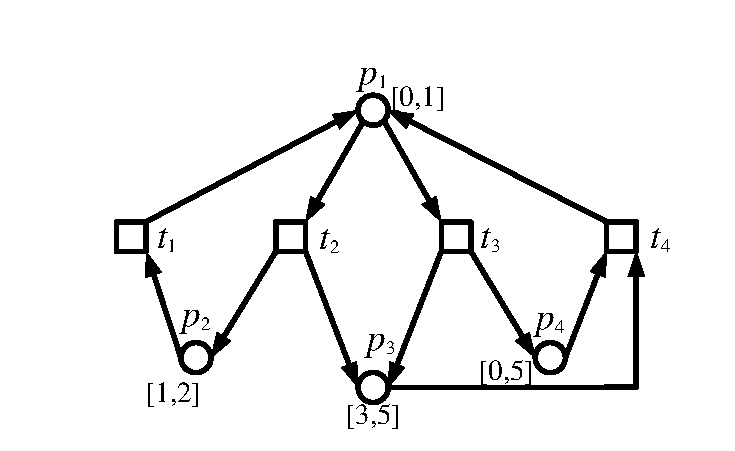
\includegraphics[scale=0.65,angle=0]{figures/figure3-2.pdf}\\
        \caption{一个TPPN模型}
    \end{figure}

    TTPN和TPPN的差异不仅仅是时间区间加在变迁或库所上这一点,他们时钟计时方式也有很大的区别。
    TTPN时钟加在变迁上,当变迁使能时,时钟开始计时,此变迁的前置库所中的托肯被更新过就会重置计时。
    而TPPN的时钟加在托肯上,会一直计时下去,托肯被移动才会重置时钟。

    基于以上的描述,TTPN和TPPN的计时方式并没有实质上的冲突,可以兼容起来。
    只需要将TTPN的变迁计时前判断库所使能的逻辑扩展为TPPN的使能逻辑就行了。
    本文为解决实际问题按此思路将TTPN和TPPN结合起来,提出了一种新的时间网子类。
\section{本章小结}
本章介绍了Petri网概念与特性、Petri网的应用、Petri网的调度方法和一系列时间网。
在接下来的章节中,将使用这些基础知识为实际系统进行建模,并使用调度算法对模型进行调度,并求解调度方案。